\subsection*{Elastica energy and the completion property}

\begin{frame}
{The elastica energy}

Let $X$ an Euclidean shape and $\alpha >0, \beta>0$.

\begin{align*}
 E(X) = \int_{\partial X}{ \alpha + \beta \kappa ^2ds}. 
\end{align*}


\end{frame}

\begin{frame}
{Completion property}
\begin{minipage}[t][0.45\textheight][t]{\textwidth}
\only<1->{
\center
$\min_{ X \subset \Omega } Data(X) + Perimeter(\partial X).$\\[1em]
}
\only<1>{
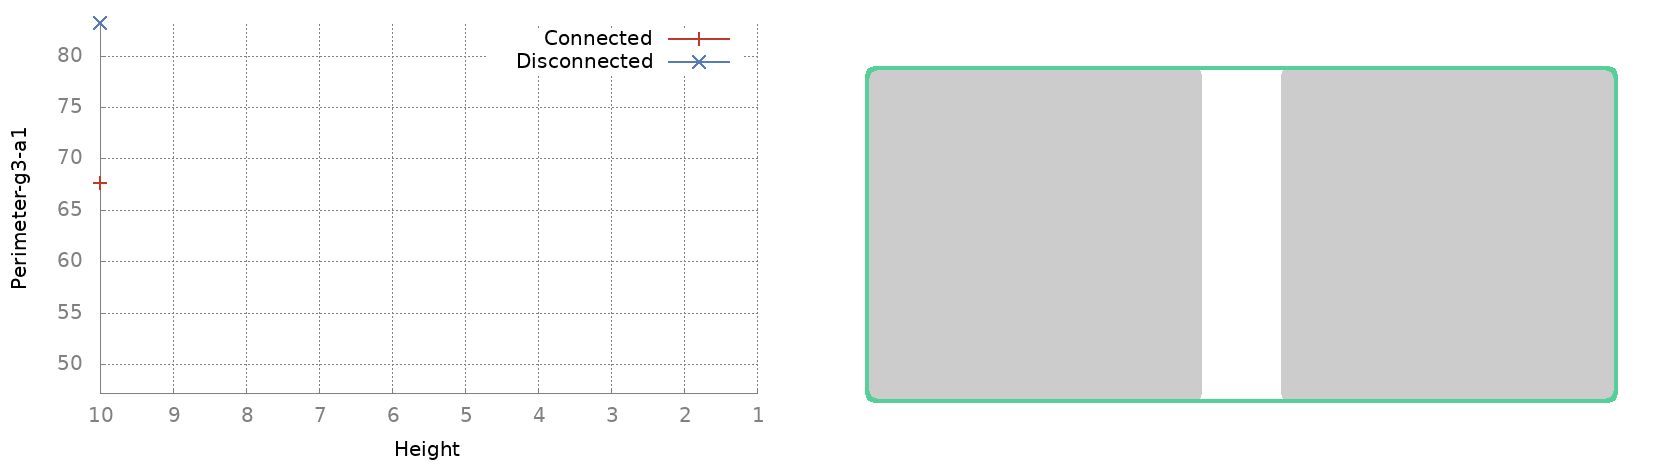
\includegraphics[scale=0.2]{figures/motivation/completion/perimeter-0.png}
}
\only<2>{
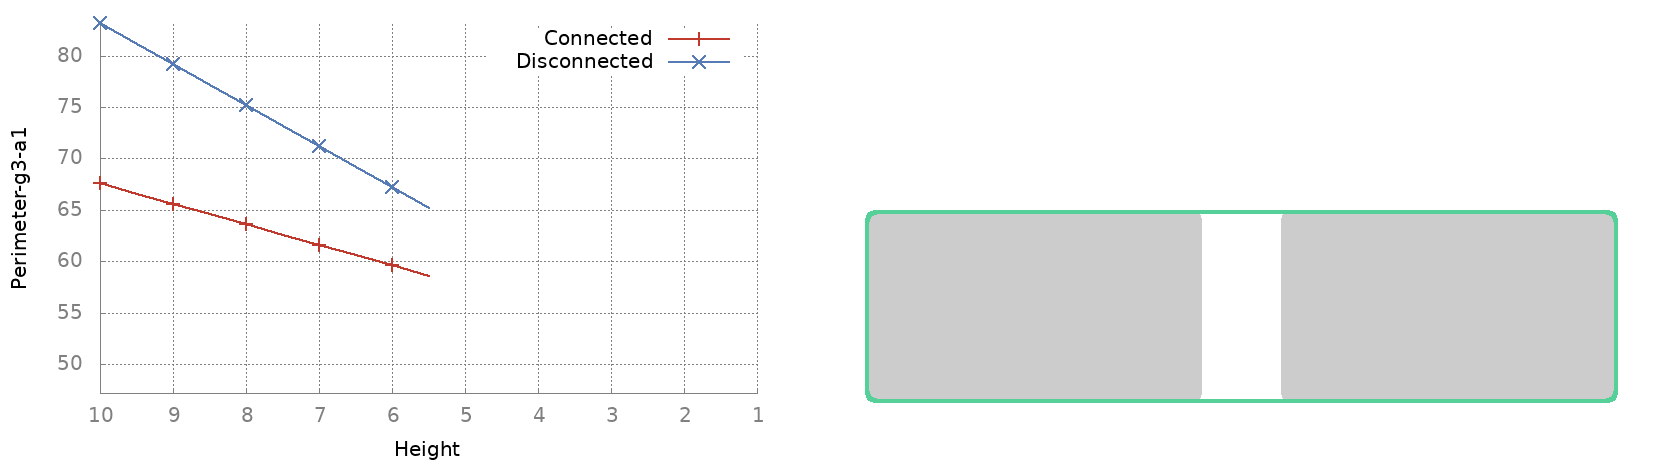
\includegraphics[scale=0.2]{figures/motivation/completion/perimeter-1.png}
}
\only<3>{
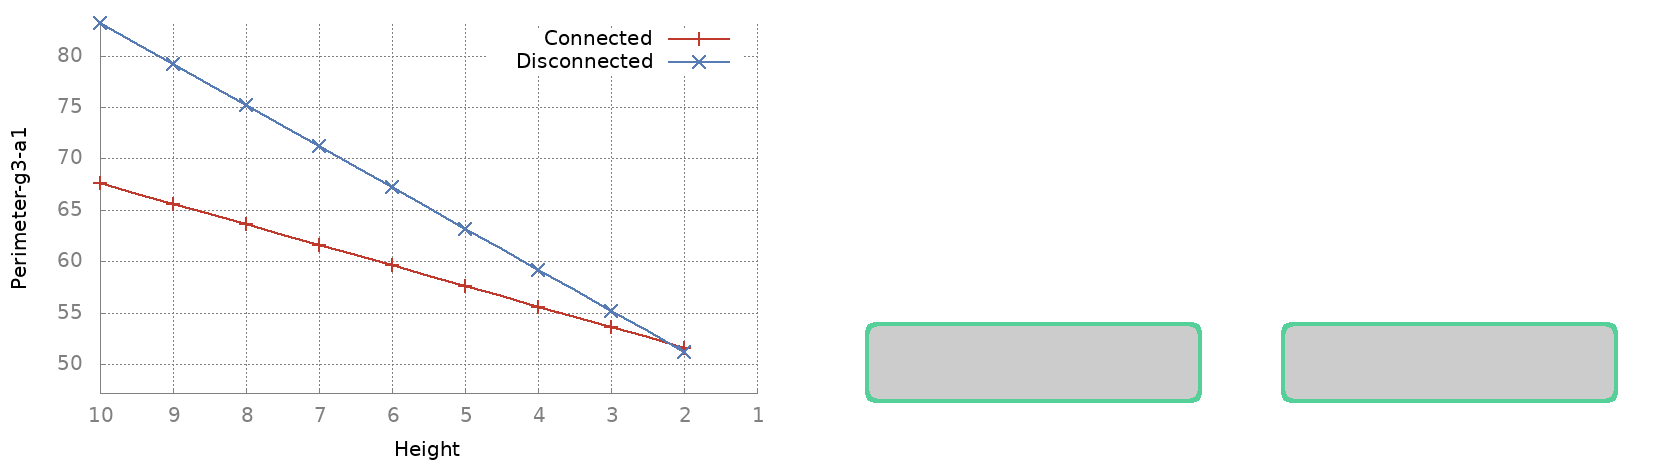
\includegraphics[scale=0.2]{figures/motivation/completion/perimeter-2.png}
}
\only<4->{
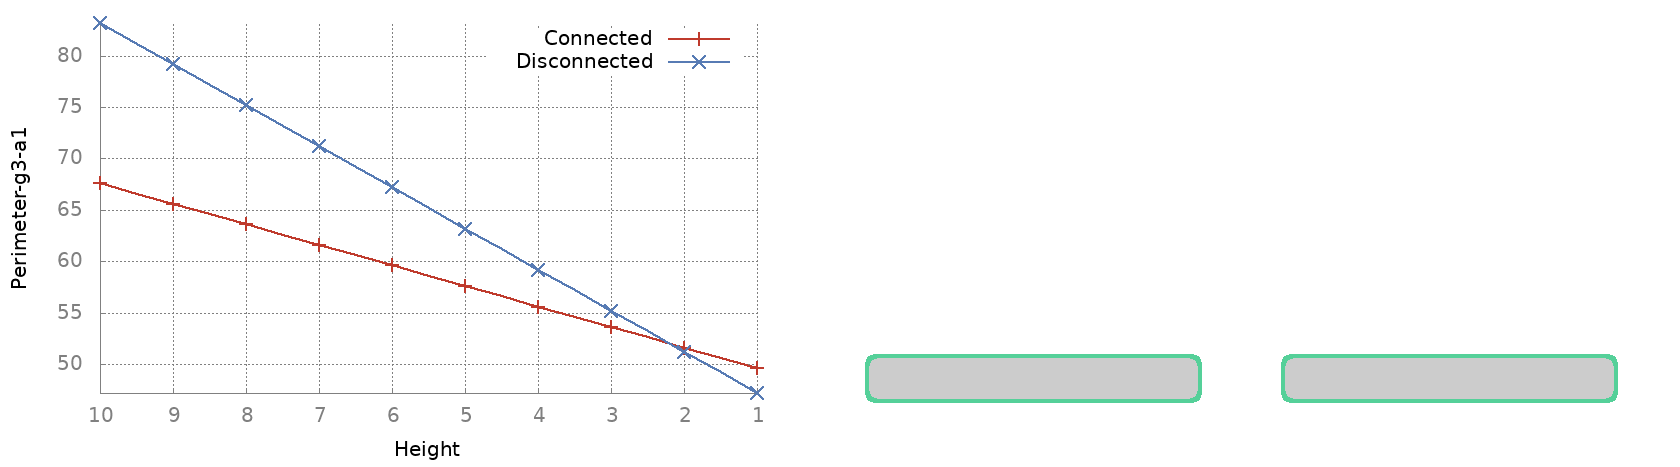
\includegraphics[scale=0.2]{figures/motivation/completion/perimeter-3.png}
}
\end{minipage}
\begin{minipage}[t][0.45\textheight][t]{\textwidth}
\only<5->{
\center
$\min_{ X \subset \Omega } Data(X) + Perimeter(\partial X) + Curvature^2(\partial X).$\\[1em]
}
\only<5>{
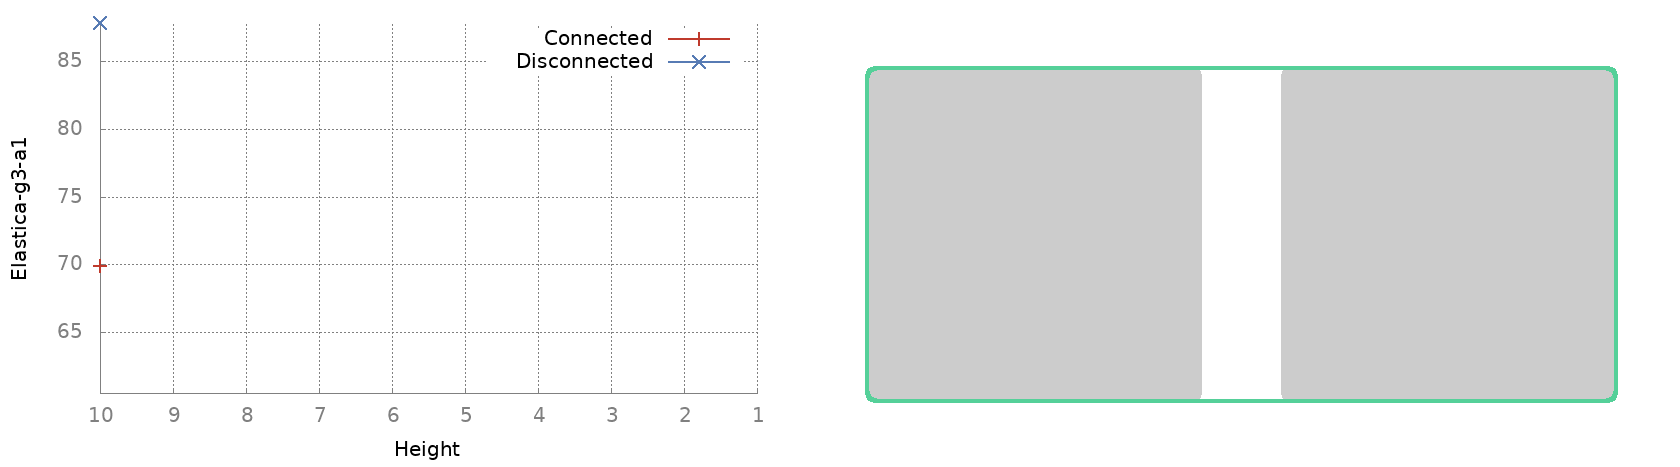
\includegraphics[scale=0.2]{figures/motivation/completion/elastica-0.png}
}
\only<6>{
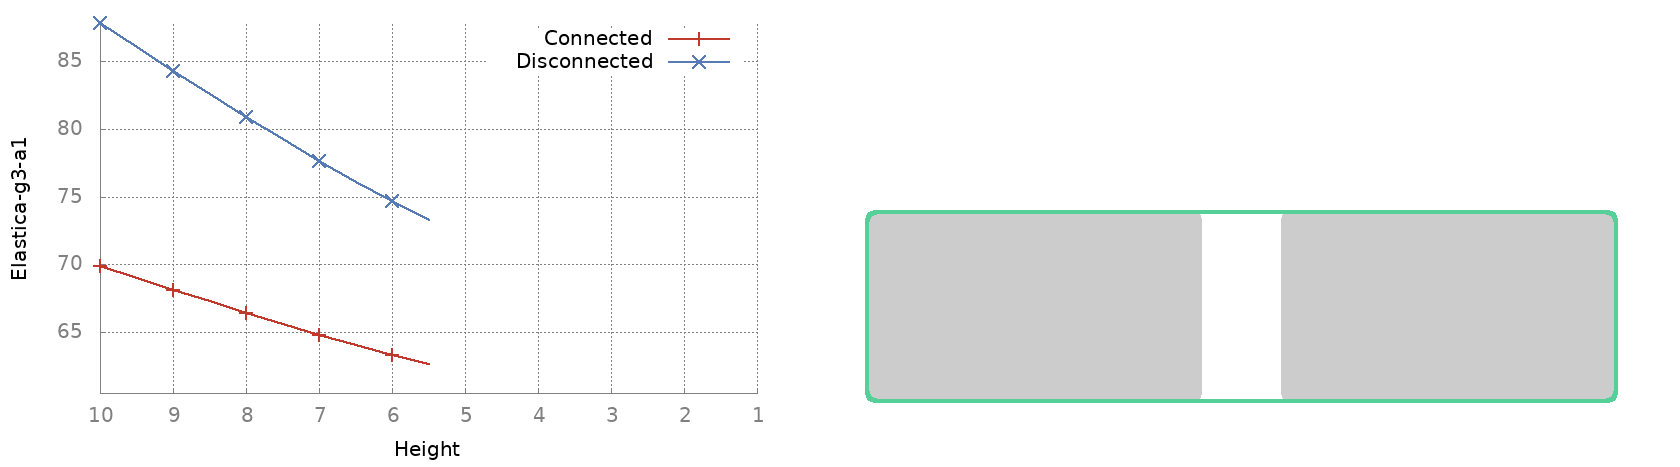
\includegraphics[scale=0.2]{figures/motivation/completion/elastica-1.png}
}
\only<7>{
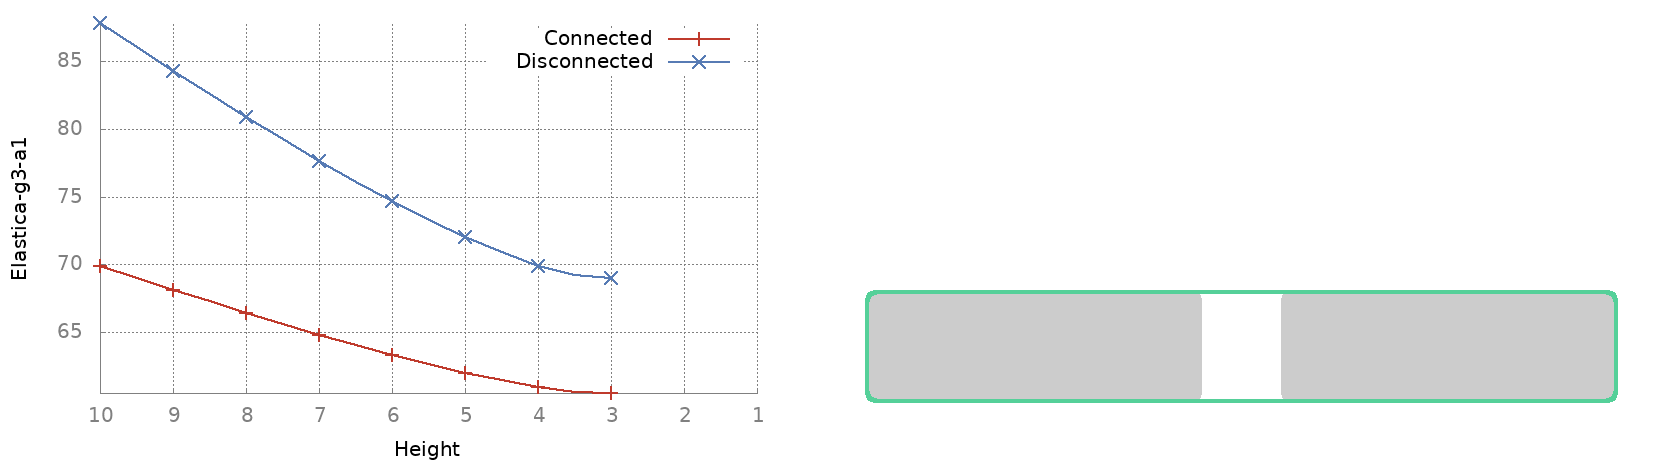
\includegraphics[scale=0.2]{figures/motivation/completion/elastica-2.png}
}
\only<8->{
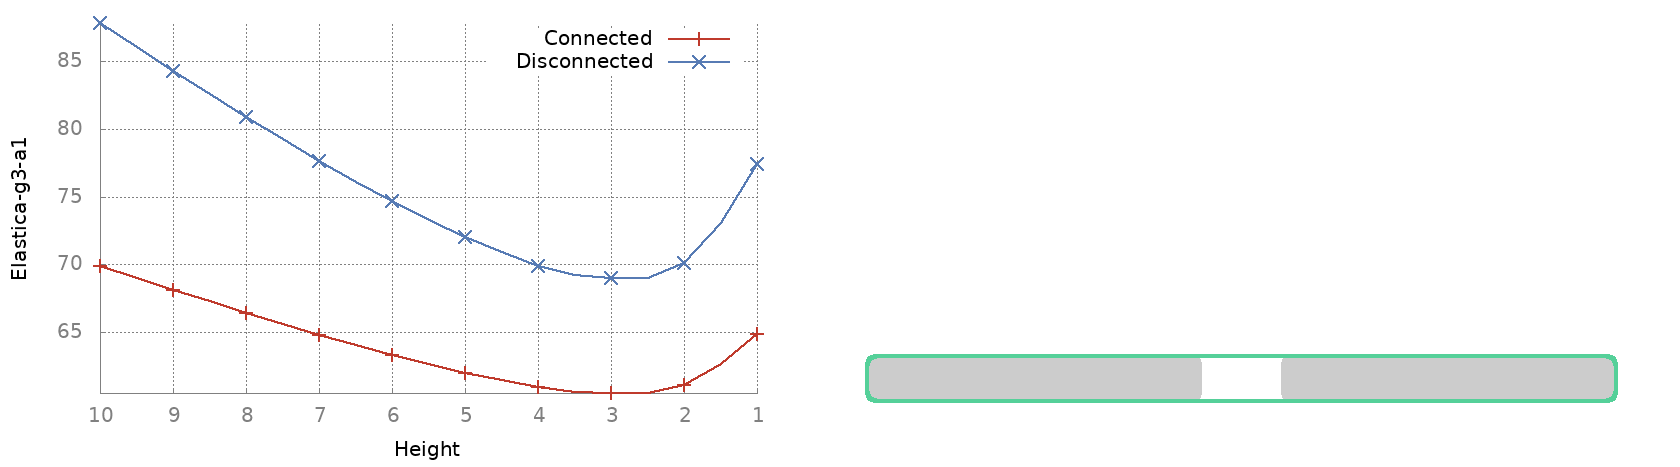
\includegraphics[scale=0.2]{figures/motivation/completion/elastica-3.png}
}
\end{minipage}
\end{frame}

\begin{frame}
{Completion property}
\begin{minipage}[t][0.45\textheight][t]{\textwidth}
\only<1->{
\center
$\min_{ X \subset \Omega } Data(X) + Perimeter(\partial X) + Curvature^2(\partial X).$\\[1em]
}
\only<1>{
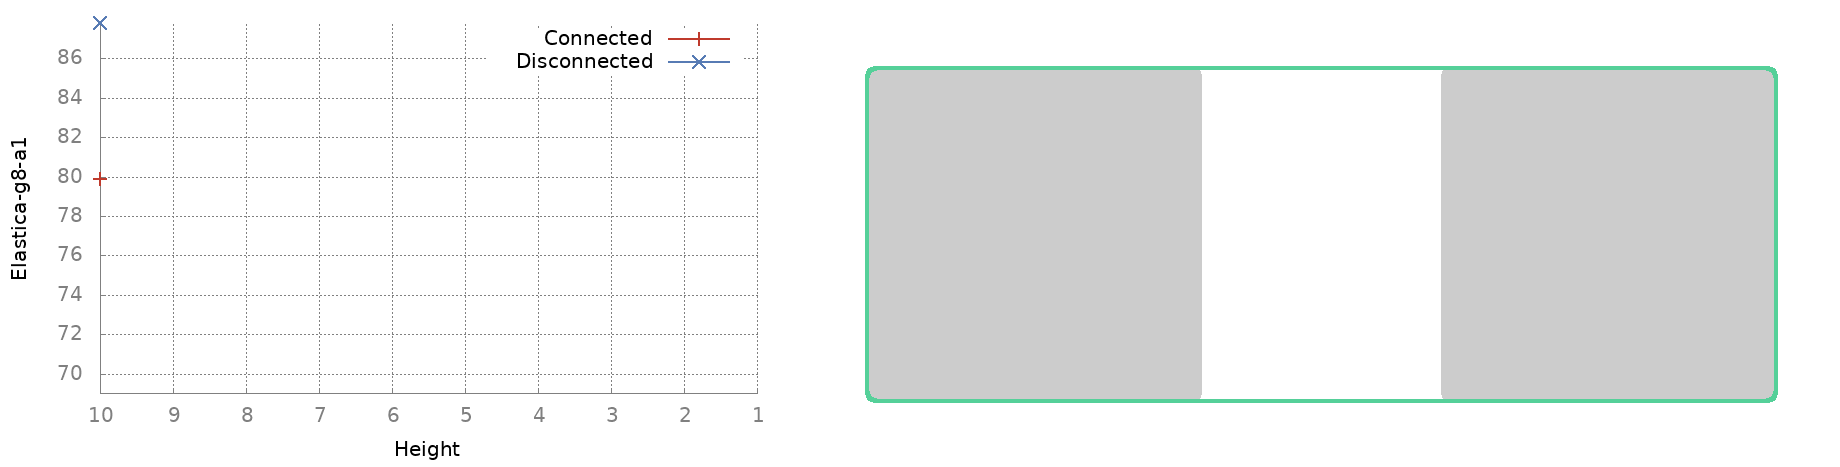
\includegraphics[scale=0.2]{figures/motivation/completion/elastica-g8a1-0.png}
}%
\only<2>{
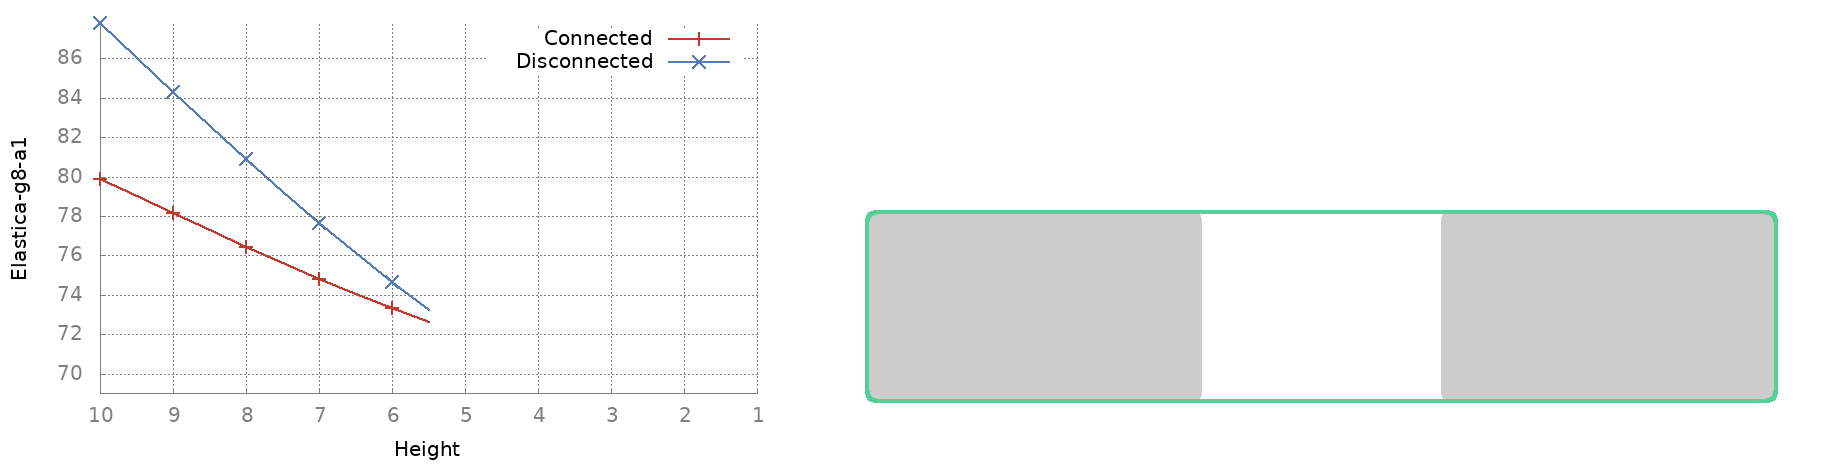
\includegraphics[scale=0.2]{figures/motivation/completion/elastica-g8a1-1.png}
}%
\only<3>{
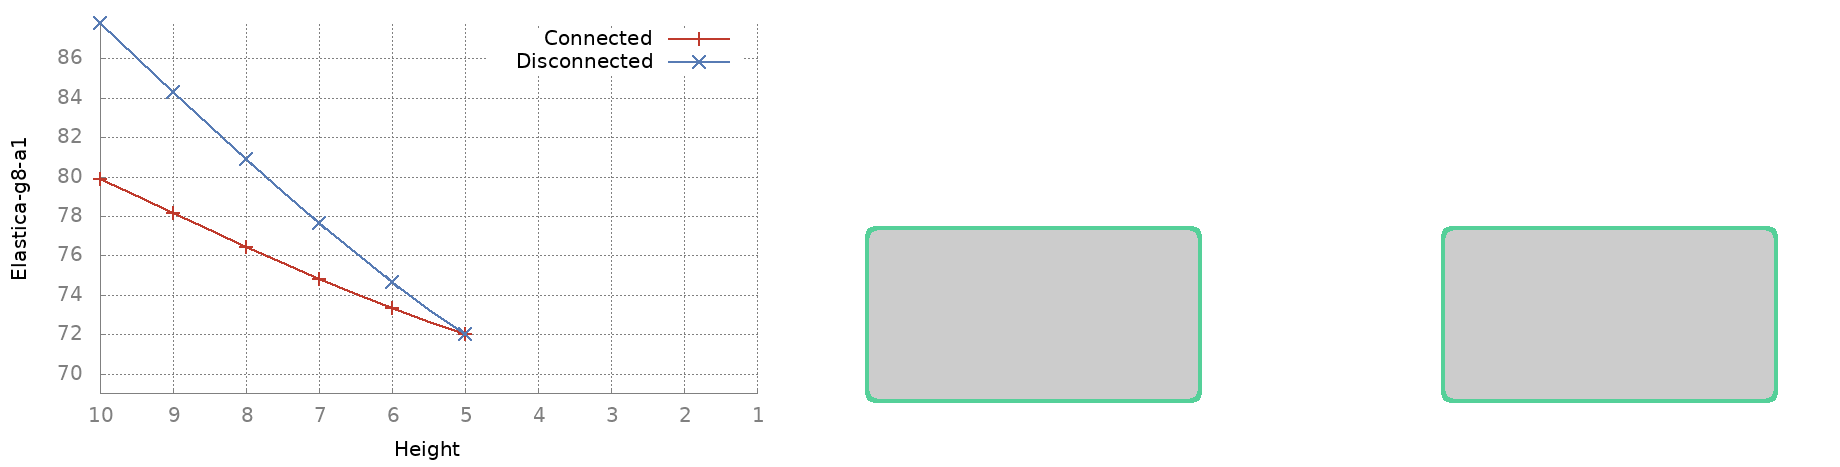
\includegraphics[scale=0.2]{figures/motivation/completion/elastica-g8a1-2.png}
}%
\only<4>{
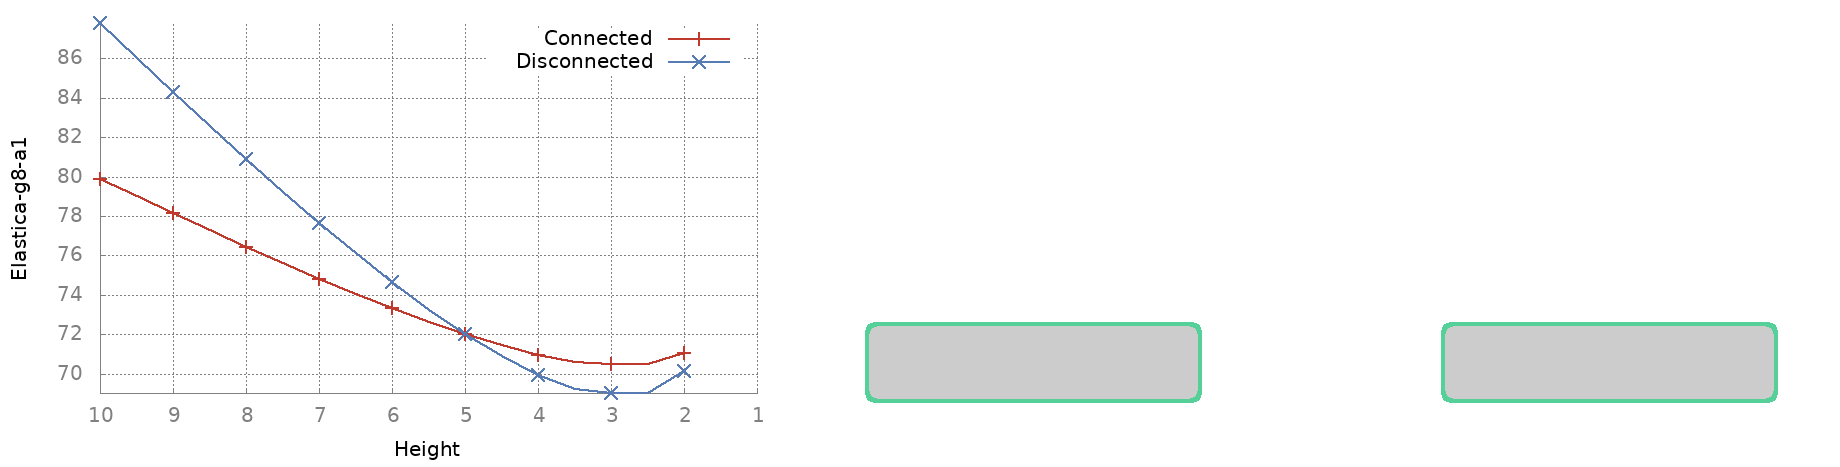
\includegraphics[scale=0.2]{figures/motivation/completion/elastica-g8a1-3.png}
}%
\only<5->{
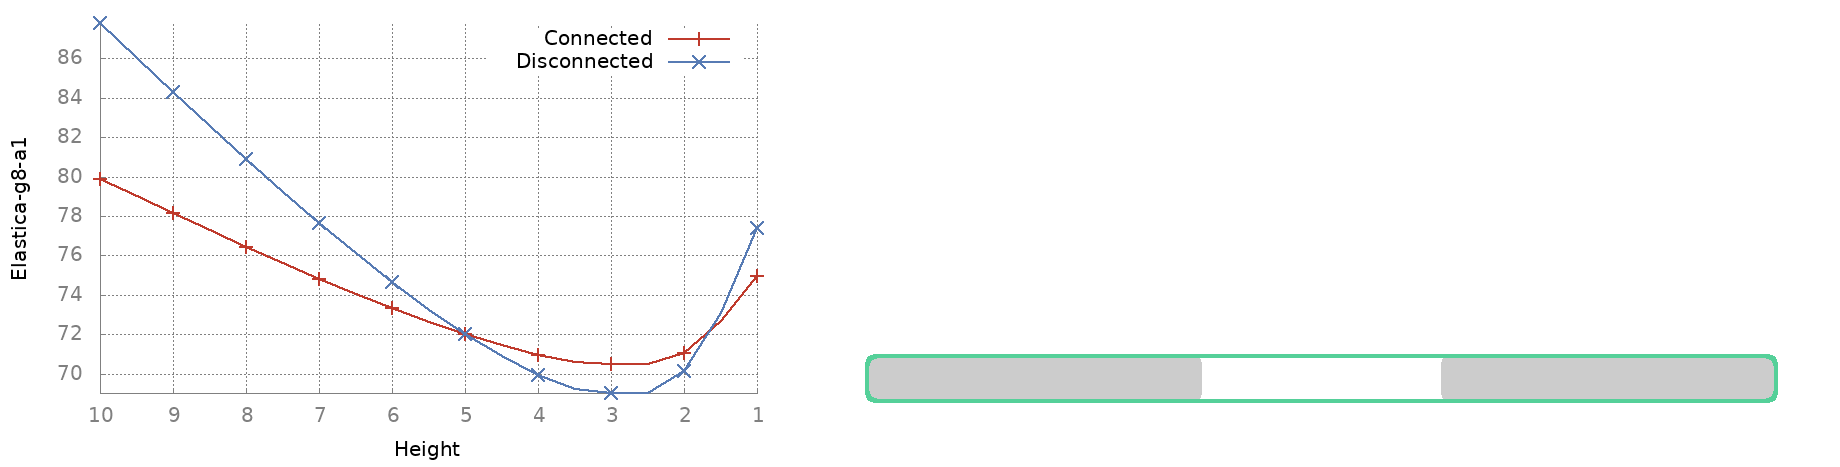
\includegraphics[scale=0.2]{figures/motivation/completion/elastica-g8a1-4.png}
}%
%
\begin{tikzpicture}
    \node at (current page.north east)
        {%
        \begin{tikzpicture}[remember picture, overlay]
		\draw [xshift=0.6cm,yshift=1.2cm,decorate,decoration={brace,amplitude=5pt,mirror,raise=4ex}]
		  (1,0) -- (2.5,0) node[midway,yshift=-3em]{Larger gap};
	  \end{tikzpicture}
	  };%
\end{tikzpicture}
%
\end{minipage}
\begin{minipage}[t][0.45\textheight][t]{\textwidth}
\only<6-10>{
\center
$\min_{ X \subset \Omega } Data(X) + {\color{highlightcolor} \frac{1}{2}} Perimeter(\partial X) + Curvature^2(\partial X).$\\[1em]
}
\only<6>{
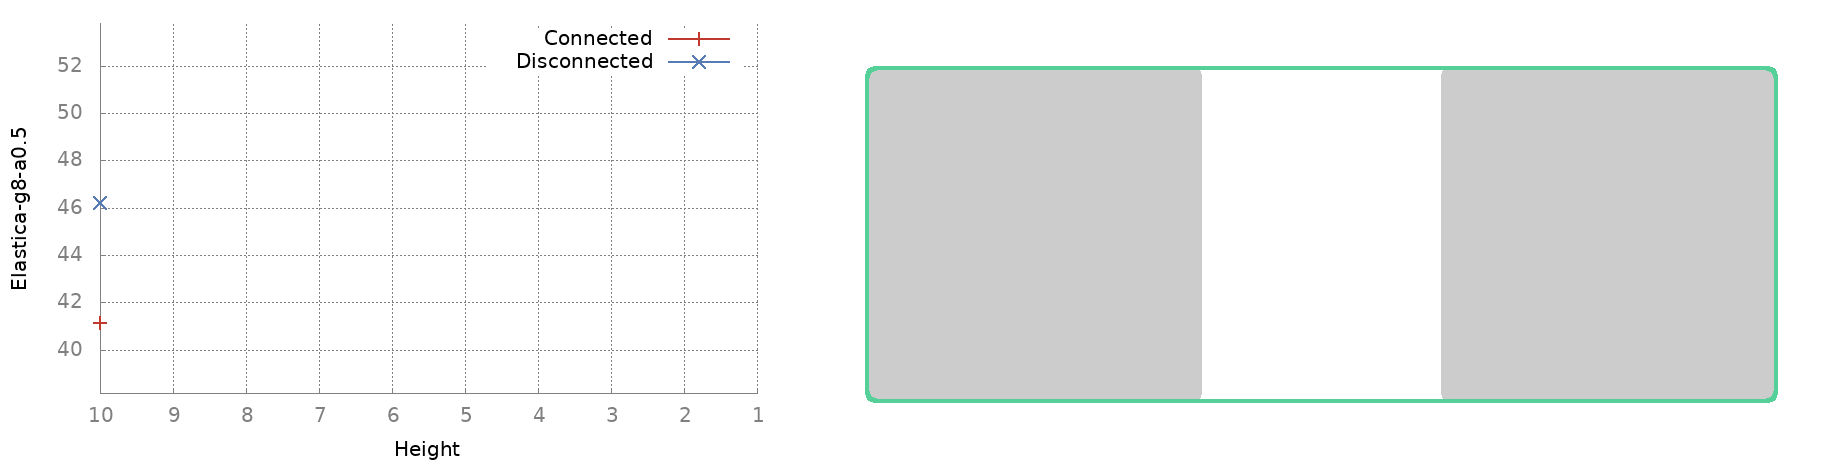
\includegraphics[scale=0.2]{figures/motivation/completion/elastica-g8a05-0.png}
}
\only<7>{
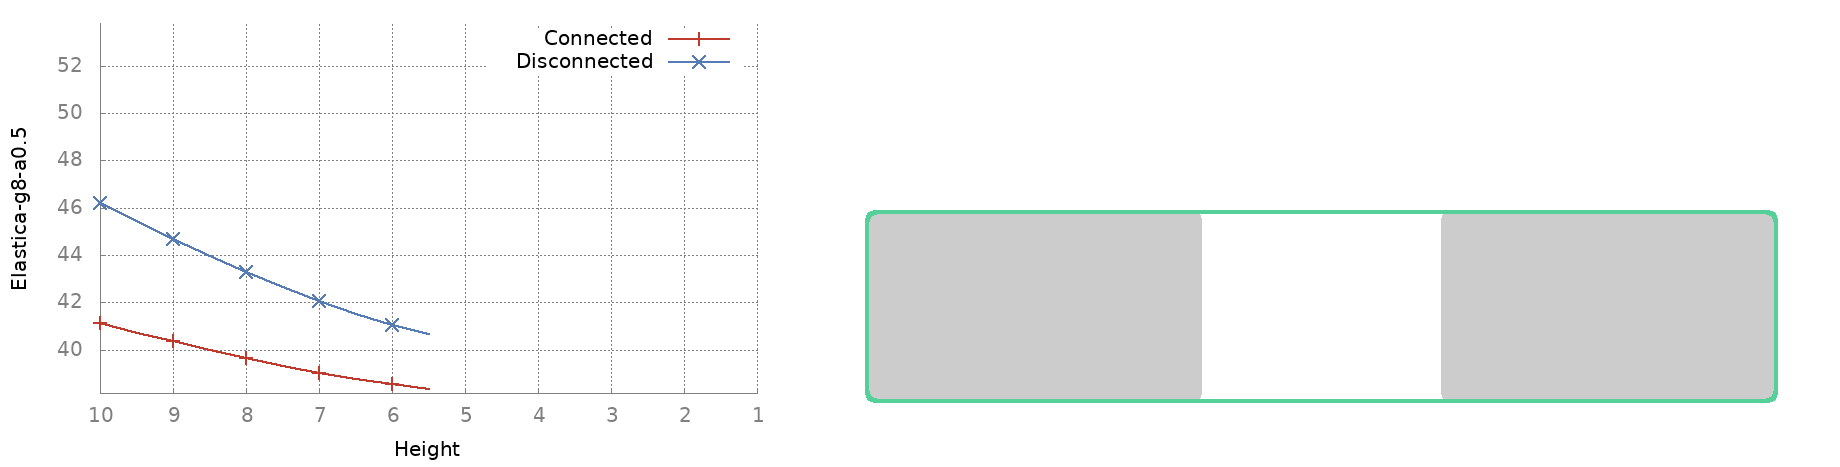
\includegraphics[scale=0.2]{figures/motivation/completion/elastica-g8a05-1.png}
}
\only<8>{
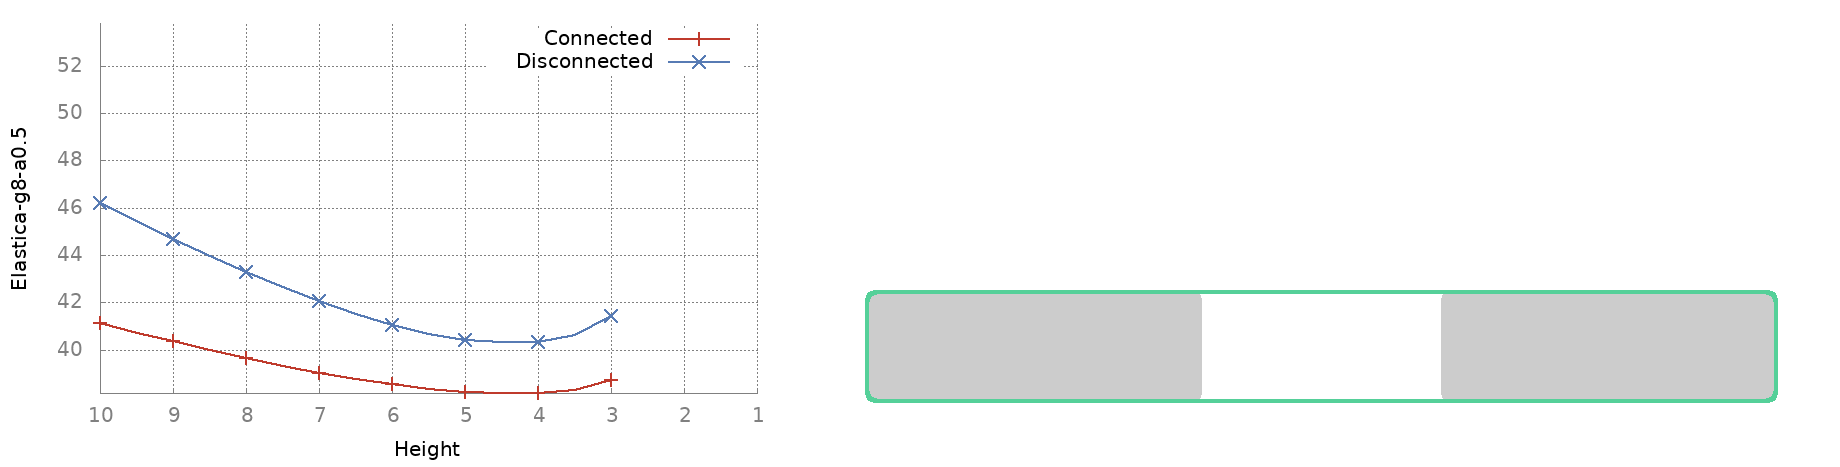
\includegraphics[scale=0.2]{figures/motivation/completion/elastica-g8a05-2.png}
}
\only<9->{
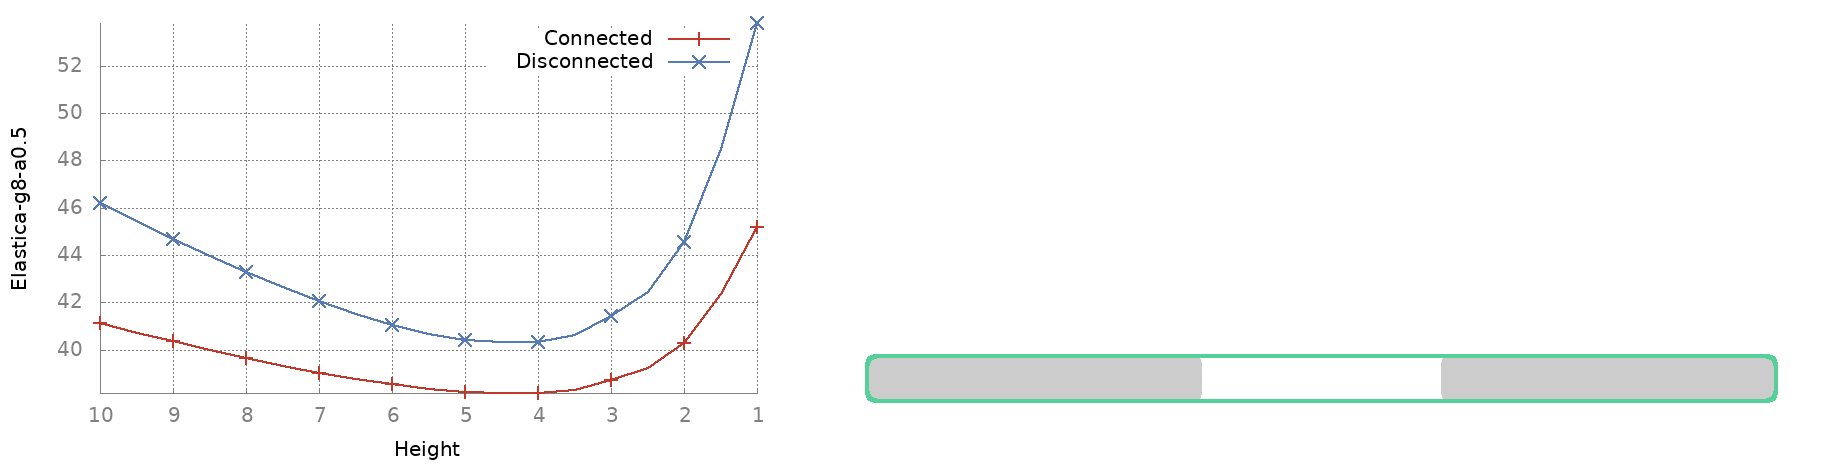
\includegraphics[scale=0.2]{figures/motivation/completion/elastica-g8a05-3.png}
}
\onslide<10>{
	\begin{figure}
	\begin{tikzpicture}[overlay, remember picture] 
	\node at (current page.center) 
	    [
	    anchor=east,
	    xshift=-10mm,
	    yshift=0mm
	    ] 
	{
	
	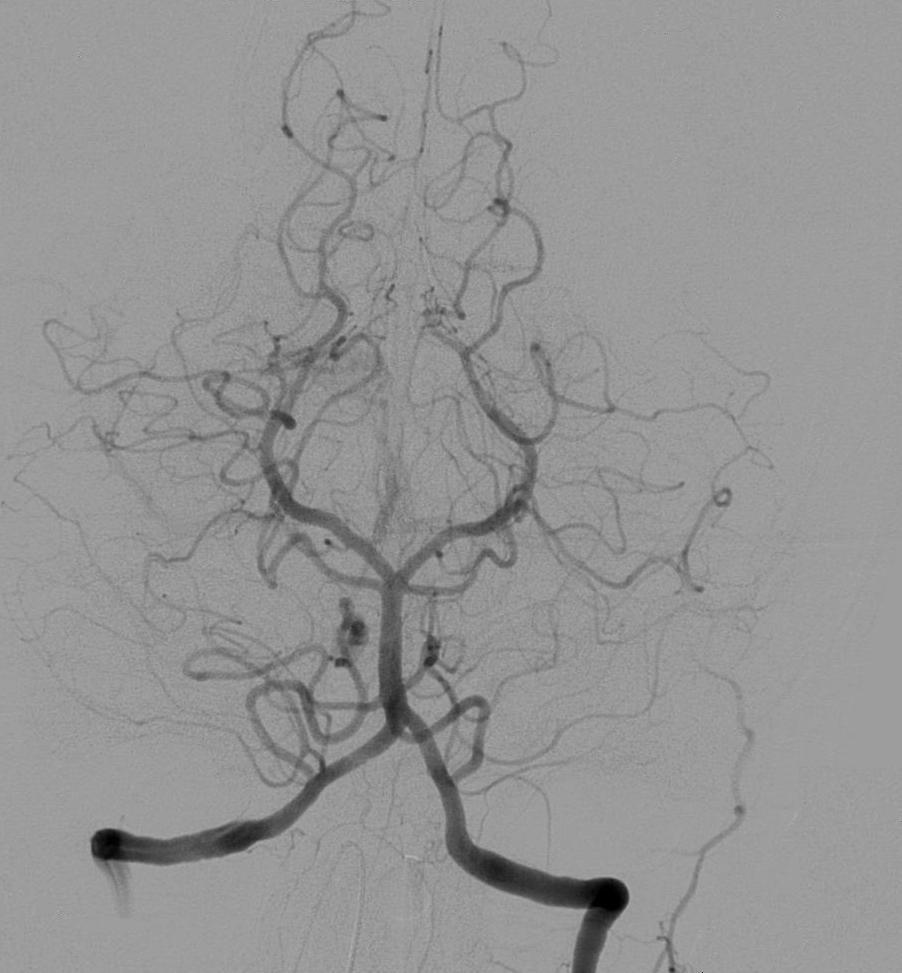
\includegraphics[scale=0.16]{figures/motivation/completion/angiogram.jpg}
		
	};
	\node at (current page.center) 
	    [
	    anchor=west,
	    xshift=-10mm,
	    yshift=0mm
	    ] 
	{
	
	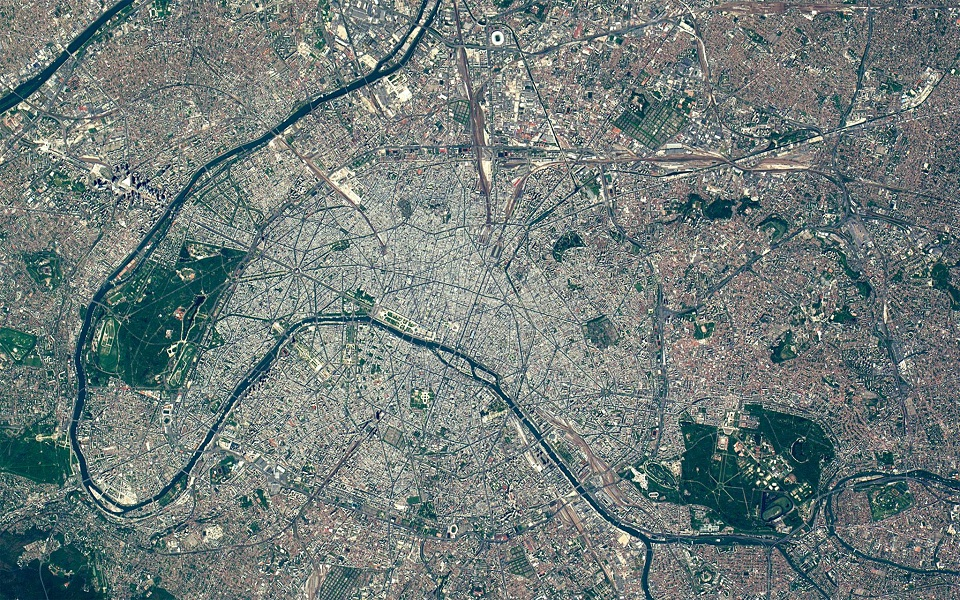
\includegraphics[scale=0.35]{figures/motivation/completion/paris-satellite-road.jpg}
		
	};	
	\end{tikzpicture}	
	\end{figure}	
	}	
\end{minipage}
\end{frame}
